\documentclass[12pt]{article}
\usepackage{a4} 
\usepackage{amsmath}
\usepackage{amssymb}
\usepackage{cite}
\usepackage{algorithm}
\usepackage[noend]{algpseudocode}
\usepackage{siunitx}
\usepackage{verbatim}
\usepackage{graphicx}
\sisetup{output-exponent-marker=\ensuremath{\mathrm{e}}}


\title{Notes on the Polar Decomposition}
\author{Michael Connolly%
        \thanks{%
                School of Mathematics,
                University of Manchester,
                Manchester, M13 9PL, England
                (\texttt{michael.connolly-6@postgrad.manchester.ac.uk}).
               }
}
\date{October, 2018}

%%%%%%%%%%%%%%%%%%%%%%%%%%%%%%%%%
\def\R{\mathbb{R}}
\def\C{\mathbb{C}}
\def\nbyn{n \times n}
\def\mbyn{m \times n}
\def\l{\lambda}
\def\norm#1{\|#1\|}      
\def\normi#1{\|#1\|_1}
\def\normo#1{\|#1\|_{\infty}}
\def\Chat{\widehat{C}}
\def\e{eigenvalue}

% \DeclareMathOperator{\diag}{diag}   % Requires amsmath.
\def\diag{\mathop{\mathrm{diag}}}     % If not using amsmath.
\def\trace{\mathop{\mathrm{trace}}}   % If not using amsmath.

\def\At{\widetilde{A}}
\def\normt#1{\|#1\|_2}

% Set up lemma environment and its numbering.
\newtheorem{lemma}{Lemma}[section]

\def\proof{\par{\bf Proof}. \ignorespaces}
\def\qedsymbol{\vbox{\hrule\hbox{%
                     \vrule height1.3ex\hskip0.8ex\vrule}\hrule}}
\def\endproof{\qquad\qedsymbol\medskip\par}

\newtheorem{theorem}{Theorem}


%%%%%%%%%%%%%%%%%%%%%%%%%%%%%%%%%%%%%%%%%%%%%%%%%%%%%%%%%%%%%%%%%%%%%%%%%%%%
% For fine-tuning spacing in \sqrt etc=.  From \cite[p.~155]{knut99}.
% In math mode, @ will act as a macro that adds 1 unit of space.
% By comparison, \, skips 3mu.

\mathcode`@="8000 % Make @ behave as per catcode 13 (active).  TeXbook p. 155.
{\catcode`\@=\active\gdef@{\mkern1mu}}
%%%%%%%%%%%%%%%%%%%%%%%%%%%%%%%%%%%%%%%%%%%%%%%%
 
%%%%%%%%%%%%%%%%%%%%%%%%%%%%%%%%%%%%%%%%%%%%%%%%%%%%%%%%%%%%%%%%%%%%%%%%%%%%
\newcounter{mylineno}
\makeatletter
\def\BState{\State\hskip-\ALG@thistlm}
\let\oldtabcr\@tabcr
\def\nonumberbreak{\oldtabcr\hspace{3.5pt}}
\def\mynewline{\refstepcounter{mylineno}%
                \llap{\footnotesize\arabic{mylineno}\hspace{5pt}}%
               }
\def\lineref#1{\footnotesize\ref{#1}}
% Next macro adapted from latex.ltx
\gdef\@tabcr{\@stopline \@ifstar{\penalty%
            \@M \@xtabcr}\@xtabcr\mynewline}
\def\myvspace#1{\oldtabcr[#1]\mynewline}
\newenvironment{code}{%
                         % Swap `:' and `colon'...
                         \mathcode`\:="603A  % TeXbook pp 134, 154, 359 (top)
% For original colon     \mathcode`\:="303A  % TeXbook p 344
                         \def\colon{\mathchar"303A}
                         \setcounter{mylineno}{0}
                         \par
                         \upshape
                         \begin{list} % To give indentation
                            {} {\leftmargin = 1cm}
                         \item[]
                         \begin{tabbing}

                         % Default tab stops
                            \hspace*{.3in} \= \hspace*{.3in} \=
                            \hspace*{.3in} \= \hspace*{.3in} \= \kill
                            \mynewline
                        }{\end{tabbing}\end{list}}
\makeatother
%%%%%%%%%%%%%%%%%%%%%%%%%%%%%%%%%%%%%%%%%%%%%%%%%%%%%%%%%%%%%%%%%%%%%%%%%%%%

\begin{document}
\maketitle

\section{Basic Properties}

We begin by defining the polar decomposition and covering some basic properties.
Let $A \in \C^{\mbyn}$ with $m \ge n$. There exists $U \in \C^{\mbyn}$ with
orthonormal columns and a unique Hermitian positive semidefinite
$H \in \C^{\nbyn}$ such that $A=UH$. $H$ is given by $(A^{*}A)^{\frac{1}{2}}$.
All $U$ are given by
\begin{equation}
  U=P
  \begin{bmatrix}
    I_r & 0 \\
    0 & W \\
  \end{bmatrix}
  Q^*\text{,}
\end{equation}
where $A = P \begin{bmatrix} \Sigma_r & 0 \\ 0 & 0_{m-r\text{, } n-r}\end{bmatrix} Q^*$
is an SVD, $r=\mathrm{rank}(A)$ and $W \in \C^{(m-r)\times (n-r)}$ is arbitrary subject
to having orthonormal columns.

We note some properties of the polar decomposition.
From this point forward we consider only square matrices.
Let $A \in \C^{\nbyn}$
have polar decomposition $A=UH$. Then:
\begin{enumerate}
\item $H=(A^*A)^{\frac{1}{2}}$,
\item $\lambda (H) = \sigma(A)$,
\item $\kappa_2(H) = \kappa_2(A)$,
\item $A$ is normal iff $UH=HU$.
\end{enumerate}

We present proofs of the second and fourth properties.
To see $\lambda(H) = \sigma(A)$, we first consider the SVD of $A$:
\begin{equation}
  A = P
  \begin{bmatrix}
    \Sigma_r & 0 \\
    0 & 0_{n-r\text{, }n-r} \\	
  \end{bmatrix} Q^*\text{,}
\end{equation}
with $P\text{, } Q \in \C^{\nbyn}$ and both unitary. $\Sigma_r$ is then a
diagonal matrix containing the singular values of $A$. We now evaluate
$A^*A = (P\Sigma Q^*)^*P\Sigma Q^* = Q\Sigma^* P^* P\Sigma Q^* = Q \Sigma^*
\Sigma Q^*$. We now note that
$H = ( Q \Sigma^* \Sigma Q^*)^{\frac{1}{2}} = ( Q \Sigma^2 Q^*)^{\frac{1}{2}}= Q
\Sigma Q^*$, as $\Sigma \in \R^{\nbyn}$. We know $\Sigma$ to be diagonal and $Q$
to be unitary, so this forms a spectral decomposition of $H$, completing the
proof.

We next show that $A^*A = AA^*$ if and only if $U$ and $H$ commute.
If $UH=HU$, then $A^*A = (UH)^*UH = H^*U^*UH = H^2 = HUU^*H = AA^*$
and we have that $A$ is normal.

If $A^*A = AA^*$, then $H^2 = UH^2U^*$. Taking the principal square root of
both sides gives $H = UHU^*$ and post-multiplying by $U$ gives the required
condition.

We next verify the formula
\begin{equation} \label{eqn:U-integral}
  U = \frac{2}{\pi}A\int_{0}^{\infty}(t^2I + A^*A)^{-1}dt\text{.}
\end{equation}
We first note that we can write $U=PQ^*$ when considering the SVD of $A$. We
can also diagonalize $A^*A = Q\Sigma^2 Q^*$, and so
\begin{equation}
  U = \frac{2}{\pi}P\Sigma Q^*\int_0^{\infty}(t^2I + Q\Sigma^2 Q^*)dt\text{.}
\end{equation}
The integrand can be manipulated in to an easily integrable expression using the
Sherman-Morrison-Woodbury matrix identity \cite{high:ASNA2}:
\begin{equation}\label{eqn:inverse}
  (A+UCV)^{-1} = A^{-1} - A^{-1}U(C^{-1} + VA^{-1}U)VA^{-1}\text{.}
\end{equation}
This of course assumes $C$ is nonsingular, which is true for $\Sigma^2$ when $A$
is full rank. Applying (\ref{eqn:inverse}), we have
\begin{align*}
  & (t^2I + Q\Sigma^2Q^*)^{-1} \\
  & = \frac{1}{t^2}I - \frac{1}{t^2}Q(\Sigma^{-2} + \frac{1}{t^2}Q^*Q)^{-1}Q^*\frac{1}{t^2} \\
  & = \frac{1}{t^2}I - \frac{1}{t^2}Q(\diag(\frac{1}{\sigma_i^2}
    + \frac{1}{t^2}))^{-1}Q^*\frac{1}{t^2} \\
  & = \frac{1}{t^2}I - \frac{1}{t^2}Q(\diag(\frac{\sigma_i^2}{\sigma_i^2 + t^2}))Q^* \\
  & = Q(\frac{1}{t^2}I - \diag(\frac{\sigma_i^2}{t^2(\sigma_i^2 + t^2)}))Q^*
    \text{, where we wrote } I = QQ^*
  \text{to factor out } Q\text{ and } Q^*\text{,}\\
  & = Q\diag(\frac{1}{\sigma_i^2 + t^2})Q^*\text{.}
\end{align*}

We can now integrate the diagonal matrix, moving the unitary matrices with no
$t$ dependence outside the integral. We have
\begin{equation}
  \int_0^{\infty}\frac{1}{\sigma_i^2+t^2}dt = \frac{\pi}{2\sigma_i}\text{,}
\end{equation}
so that the matrix integral reads $(\pi /2)\Sigma^{-1}$.
Finally, collecting all terms we have:
\begin{align*}
  U & = \frac{2}{\pi}P\Sigma Q^*Q\frac{\pi}{2}\Sigma^{-1}Q^* \\
    & = PQ^* \text{ as required.}
\end{align*}

\section{Numerical Methods}
\subsection{Newton Iteration}
Given that $U^*U = I$, we consider the equation $(X+E)^*(X+E) = I$, with $E$ a
first order perturbation.
\begin{align*}
  (X+E)^*(X+E) & = I\text{, } \\
  X^*X + X^*E + E^*X & = I\text{, where we drop the } E^2 \text{ term,} \\
  X^*E + E^*X &  = I - X^*X\text{.} 
\end{align*}
Promoting $X$ and $E$ to be members of a sequence, we obtain:
\begin{align}\label{eqn:newtonderiv}
    X_k^*E_k + E_k^*X_k & = I - X_k^*X_k\text{,} \\
    X_{k+1} & = X_k + E_k\text{.}
\end{align}
Writing $E_k = (X_k^{-*} - X_k)/2$, and substituting for
$E_k$ in (\ref{eqn:newtonderiv}), we obtain:
\begin{align*}
  &\frac{1}{2}X_k^*(X_k^{-*} - X_k) + \frac{1}{2}(X_k^{-1} - X_k^*)X_k \\
  &= \frac{1}{2}I - \frac{1}{2} X_k^*X_k + \frac{1}{2}I -  \frac{1}{2} X_k^*X_k  \\
  &= I - X_k^*X_k\text{.}
\end{align*}
$E_k$ of this form thus satisfies (\ref{eqn:newtonderiv}) and so we arrive
at the Newton Iteration for the unitary polar factor $U$:
\begin{equation}\label{eqn:newton}
  X_{k+1} = \frac{1}{2}(X_k + X_{k}^{-*})\text{, } X_0 = A\text{.}
\end{equation}

We analyse the convergence of the Newton Iteration by considering the SVD of $A$.
As previously noted, we have that $A=P\Sigma Q^*$ and $U=PQ^*$.
We postulate that $X_k = PD_kQ^*$, with $D_{k+1} = (D_k + D_k^{-1})/2$, $D_0 = \Sigma$.
The proof is by induction.
It is trivially true for $X_0$ as $D_0 = \Sigma$.
For $X_1$, we have that $X_1 = (A + A^{-*})/2$.
The equivalence between the two is immediate:
\begin{equation*}
  PD_1Q^* = \frac{1}{2}(P\Sigma Q^* + P\Sigma^{-1} Q^*) = \frac{1}{2}(A + A^{-*}) = X_1\text{.}
\end{equation*}
Assuming it to be true that $X_k = PD_kQ^*$, we consider:
\begin{align*}
  X_{k+1} & = \frac{1}{2}P(D_k + D_k^{-1})Q^* \\
          & = \frac{1}{2}PD_kQ^* + \frac{1}{2}PD_k^{-1}Q^* \\
          & = \frac{1}{2}(X_k + X_k^{-*})\text{, }
\end{align*}
which is of course the Newton Iteration. The $D_k$ iteration is the Newton
Iteration for $\mathrm{sign}(\Sigma) = I$, which we know to be true as $\Sigma$
is diagonal with positive entries. These Newton iterates $D_k$ thus converge
quadratically to $I$\cite{Higham:2008:FM}.

Moreover, we can consider:
\begin{align*}
  X_{k+1} - U & = \frac{1}{2}(PD_kQ^* - PQ^* + PD_k^{-1}Q^* - PQ^*) \\
  & = \frac{1}{2}(PD_kQ^* - PQ^*)QD_k^{-1}P^*(PD_kQ^* - PQ^*)\\
  & = \frac{1}{2}(X_k - U)X_k^{-1}(X_k - U)\text{.}
\end{align*}
We thus have the relation
\begin{equation}
  \norm{X_{k+1} - U} \leq \frac{1}{2}\norm{X_k^{-1}}\norm{X_k - U}^2\text{.}
\end{equation}

\subsection{Newton-Schulz Iteration}
We derive an alternative iterative method to the Newton Iteration. We remove
the inverse from the formula by approximating it with one step of Newton's
method for the matrix inverse:
\begin{equation}
  Y_{k+1} = Y_k(2I - BY_k)\text{,}
\end{equation}
for computing $B^{-1}$. Replacing $X_k^{-*}$ by $X_k(2I - X_k^*X_k)$ in
(\ref{eqn:newton}), having taken $X_k^* = B$, $Y_k = X_k$, we obtain the
Newton-Schulz iteration:
\begin{equation}
  X_{k+1} = \frac{1}{2}X_k(3I - X_k^*X_k)\text{, } X_0 = A\text{.}
\end{equation}
The convergence of the Newton-Schulz iteration can be analyzed in a similar
fashion to the Newton iteration. By considering the SVD of $A$ we again write
$X_k = PD_kQ^*$ with $D_{k+1} = D_k(3I - D_k^2)/2$, with $D_0 = \Sigma$. Again,
we show this by induction. It is once again trivial for $X_0 = A$,
$D_0 = \Sigma$. For $k = 1$, we have that $D_1 = \Sigma(3I - \Sigma^2)/2$. The
required result follows easily:
\begin{align*}
  X_{1} & = \frac{1}{2}P\Sigma(3I-\Sigma^2)Q^* \\
          & = \frac{3}{2}P\Sigma Q^* - \frac{1}{2}P\Sigma^3Q^* \\
          & = \frac{3}{2}X_0 - \frac{1}{2}X_0X_0^*X_0 \\
  & = \frac{1}{2}X_0(3I - X_0^*X_0)\text{, as required.}
\end{align*}
Note in the penultimate step we made use of the fact that
$X_0X_0^*X_0 = P\Sigma^3Q^*$, which is trivial to show. We then assume that
$X_k = PD_kQ^*$. Writing
$PD_{k+1}Q^* = PD_k(3I - D_k^2)Q^*/2 = 3X_k/2 - (PD_k^3Q^*)/2$, it only remains
to be shown that $X_kX_k^*X_k = PD_k^3Q^*$. Exploiting the fact that $D_k$ is
diagonal with real entries, we can write $X_k^*X_k = QD_k^2Q^*$. We obtain the
required expression by writing $PD_k^3Q^* = PD_kQ^*(QD_k^2Q^*) = X_kX_k^*X_k$.

Given that $D_k = \diag(d_k^i)$, the entries of $\diag(d_k^{i})$ are given by
$d^{i}_{k+1} = f(d^{i}_k)$, $f(x) = x(3-x^2)/2\text{, } d_0^{i} = \sigma_i$. So
in order for $D_k \to I$, the singular values of $A$ must all lie in the region
in which the mapping $x_{n+1} = f(x_n)$ is stable and has a fixed point of $1$.
The fixed points of an iterative map are those for which $x = f(x)$, given here
by $x = 0\text{, }\pm 1$.
Consider first $x_n \in (0, 1)$.
We have $f(0) = 0\text{, } f(1) = 1$ and $f^{\prime}(x) < 0$ for $x \in [0, 1)$.
The $x_n$ thus form a sequence tending to a limit in $[0, 1]$,
which must be the fixed point $1$.
For $x_n \in (1\text{, } \sqrt{3})$, we have $f(1) = 1$,
$f(\sqrt{3}) = 0$ and $f^{\prime}(x) < 0$ for $x > 1$.
As a result $f$ maps $(1, \sqrt{3}) \to (0, 1)$ and after the first iteration
we can apply the previous argument.
$\lvert f^{\prime}(x) \rvert$ informs us about the
stability of a fixed point. A fixed point $x^*$ is stable, i.e. an attractor,
if $\lvert f^{\prime}(x^*) \rvert < 1$, and unstable, i.e. a repellor, if
$\lvert f^{\prime}(x^*) \rvert > 1$. For this map we have that $x^* = \pm 1$
are attractors and $x^* = 0$ is a repellor. The region in which we are
interested is that for which we reach the fixed point $1$. It is easy to see
that this is $0 < x_0 < \sqrt{3}$. For $x_0 = 0\text{, } \sqrt{3}$ we reach
$x^* = 0$. For $x_0 > \sqrt{3}\text{, } x_1 < 0$ and so we reach $x^* = -1$.
We thus require the diagonal entries of $\Sigma$ to all be non-zero and less
than $\sqrt{3}$ for the Newton-Schulz iteration to converge. We could
alternatively phrase this as $A$ being non-singular and $\norm{A}_2 < \sqrt{3}$.
This result can be shown more generally for the iterative map:
\begin{equation}
  y_{k+1} = \frac{1}{p}[(1+p)y_k - y_k^{p+1}] = f(y_k)
  \text{, } y_0 = a^{1/p}\text{.}  
\end{equation}
It can be shown \cite{Higham:2008:FM} that $y_k \to 1$ if $y_0 < (p+1)^{1/p}$,
and so the Newton-Schulz iteration reduces to the $p=2$ case.

Considering the quantity $(X_k - U)(X_k+2U)^*(X_k-U)$, we diagonalize it using
the SVD as usual. We can then write
\begin{align*}
  & (PD_kQ^* - PQ^*)(QD_kP^* + 2QP^*)(PD_kQ^* - PQ^*)\\
  & = (PD_k^2P^* + 2PD_kP^* - PD_kP^* - 2I)(PD_kQ^* - PQ^*)\\
  & = PD_k^3Q^* - 3PD_kQ^* + 2PQ^*\text{.}
\end{align*}
We have that $X_kX_k^*X_k = PD_k^3Q^*$ and so
\begin{math}
  \frac{1}{2}(X_k - U)(X_k+2U)^*(X_k-U)
  = -\frac{1}{2}(X_k(3I-X_k^*X_k) - 2U) = -(X_{k+1}-U)
\end{math}
so that finally we have the relation:
\begin{equation}
  \norm{X_{k+1}-U}_2 \leq \frac{1}{2}
  \norm{X_k+2U}_2\norm{X_k - U}_2^2\text{.}
\end{equation}
We can also consider the convergence of the Newton-Schulz iteration in
terms of the residual $R_k = I-X_k^*X_k$. This satisfies \cite{Higham:2008:FM}
\begin{equation*}
  R_{k+1} = \frac{3}{4}R_k^2 + \frac{1}{4}R_k^3\text{.}
\end{equation*}
Thus for $\norm{R_k} < 1$, we have
$\norm{R_{k+1}} < 3\norm{R_k}^2/4 + \norm{R_k}^2/4 = \norm{R_k^2} < \norm{R_k}$,
and so the $\|R_k\|$ form a sequence converging to zero. This later provides us
with an important test on the convergence of the Newton-Schulz method.

\subsection{Computational Cost}
We now consider the operation count of the Newton and Netwon-Schulz iterations,
where $A \in \C^{\nbyn}$. The operation count for the Newton iteration is
$2n^3 + \mathcal{O}(n^2)$, assuming the matrix inverse is computed by Gaussian
elimination with partial pivoting (GEPP), making each iteration
$\mathcal{O}(n^3)$. Writing the Newton-Schulz iteration as
$X_{k+1} = (3/2)X_k - (1/2)X_kX_k^*X_k$, we see that the cost is $3n^2$ (two
matrices multiplied by scalars plus a matrix subtraction, each of cost $n^2$),
plus the cost of forming the matrix product $X_kX_k^*X_k$. We can take
advantage of the fact that the product $X_k^*X_k$ forms a symmetric matrix, so
that in computing this product we only need to compute either the upper or lower
triangular part of the matrix. With each entry in the resultant triangular
matrix costing $2n-1$ operations to compute, the cost of this is then
$(2n-1)\Sigma_{i=1}^n i = 2n(n-1)(n+1)/2 = n^3 - n$ operations. We have another
$2n^3$ operations from the subsequent matrix product, meaning the total cost of
the Newton-Schulz iteration is $3n^3 + \mathcal{O}(n^2)$, again
$\mathcal{O}(n^3)$. Ignoring total operation counts, we see that we perform one
matrix inversion in the Newton iteration, compared to two matrix multiplications
in the Newton-Schulz iteration. This means we require matrix multiplication to
be twice as fast as inversion in order for the Newton-Schulz iteration to be
quicker, or $1.5$ times as fast if we take advantage of the symmetry in the
matrix product.

\section{Experiments and Results}
In order to practically compute the polar decomposition, we employ an algorithm
wherby we start with the Newton iteration and switch to the Newton-Schulz
iteration when it's convergence is guaranteed. The motivation for this is that
the Newton-Schulz iteration is multiplication rich, which is very fast on high
performance computers. We switch to the Newton-Schulz iteration when
$\normo{I - X_k^*X_k} \leq \theta$, for some $\theta < 1$.

The termination criteria we employ are:
\begin{equation*}
  \delta_{k+1} < \eta \text{ or } \delta_{k+1} > \delta_k /2\text{, }
\end{equation*}
where $\delta_{k+1} = \normo{X_{k+1} - X_k}/\normo{X_{k+1}}$. $\eta$ is the
desired relative error to which we assign a value of $n^{1/2}u$, with $u$ the
unit roundoff. Another point to note is that upon computing $\hat{U}$, we
compute $\hat{H} = (H^{\prime} + (H^*)^{\prime})/2$ with
$H^{\prime} = \hat{U}^*A$. This guarantees that $\hat{H}$ is Hermitian.

\begin{algorithm}
  \caption{Polar Decomposition}\label{polar_decomp}
  \begin{algorithmic}[1]
    \State $X_0 \gets A$; switch $\gets$ false
    \For{$k = 0:\infty$}
    \If{not switch}
    \If{$\normo{I-X_k^*X_k} \leq \theta$}
    \State switch $\gets$ true
    \EndIf
    \EndIf

    \If{switch}
    \State $X_{k+1} \gets X_k(3I - X_k^*X_k)/2$
    \Else
    \State $X_{k+1} \gets (X_k + X_k^{-*})/2$
    \EndIf
    \State $\delta_{k+1} \gets \normo{X_{k+1} - X_k}/\normo{X_{k+1}}$
    \If{$\delta_{k+1} \leq \eta \text{ or } \delta_{k+1} > \delta_k/2$}
    \State break
    \EndIf
    \EndFor
    \State $U \gets X_{k+1}$
    \State $H \gets U^*A$
    \State $H \gets \frac{1}{2}(H + H^*)$
  \end{algorithmic}
\end{algorithm}

We present the results of this algorithm on various test matrices. We chose
$\theta$ to be $0.7$, but we note that the choice of any reasonable $\theta$ did
not have a significant effect on the algorithm.
\begin{table}
  \caption{Numerical results on test matrices} \label{tab:res}
  \begin{center}
    \begin{tabular}{| l | c | c | c | c |}
      \hline
      $A$ & $k+1$ & $\delta_{k+1}$ & $\frac{\normo{A-\hat{U}\hat{H}}}{\normo{A}}$
      & $\normo{I - X_{k+1}^*X_{k+1}}$ \\ \hline
      \texttt{randn(10)} & $9$ & \num{1.5e-16} & \num{3.2e-16} & \num{5.6e-16} \\
      \texttt{eye(8)} & 1 & 0 & 0 & 0 \\
      \texttt{hilb(6)} & 29 & \num{1.1e-16} & \num{0} & \num{7.7e-34} \\
      \texttt{magic(6)} & 59 & \num{1.5e-16} & \num{0.052} & \num{8.0e-16} \\
      \texttt{hadamard(8)} & 8 & \num{1.4e-16} & \num{2.5e-16} & \num{4.0e-16}\\
      \hline
    \end{tabular}
  \end{center}
\end{table}

$\mathcal{N}(0, 1)$\textit{ matrices:} In order to test the algorithm, we
computed the polar decomposition of matrices of various sizes, with entries
sampled from $\mathcal{N}(0, 1)$. For a sample matrix with $n=10$, the algorithm
switches to the Newton-Schulz iteration after $3$ iterations and terminates
after $9$ iterations.

\textit{Identity matrix:} For $I_8$ the iteration terminates immediately as
expected, given that the Newton or Newton-Schulz iteration applied to the
identity computes itself. The computed polar factors are again identity
matrices, which of course satisfy the required properties of $U$ and $H$.

\textit{Hilbert matrix:} For the ill-conditioned Hilbert matrix with
$\kappa_2 = 1.4951\times 10^7$ the algorithm requires $29$ iterations for
convergence and only switches to the Newton-Schulz iteration after the $24$th
iteration. Upon terminating, we have $\delta_{k+1} = \num{1.1e-16}$. The
computed answer is accurate. We also have $\hat{U} = I$ and so $\hat{H} = A$.
This is expected given that $A$ is symmetric. As such the SVD is equivalent to
a spectral decomposition and $U = PQ^* = I$.

\textit{Magic Square:}
The performance on the rank deficient $6\times 6$ magic
square is poor as expected. It requires $59$ iterations to converge, yet even
upon reforming $A$ from $\hat{U}\hat{H}$, we can see by inspection that the
entries are inaccurate by order $10^{-1}$. We also have that
$\normo{A - \hat{U}\hat{H}}/\normo{A} = 0.0052$ and not of order $\eta$ as we
would hope. This behaviour is of course entirely expected given that
\texttt{magic(6)} is singular and we attempt to compute it's inverse in the
Newton iteration.

\textit{Hadamard matrix:} For the perfectly conditioned $8\times 8$ Hadamard
matrix, we terminate after the $8$th iteration, switching to the Newton-Schulz
iteration at the $3$rd. We note that $\hat{H} = \alpha I$, with
$\alpha = 2.248$. This is a verification of $\lambda(H) = \sigma(A)$, as can be
seen by evaluating \texttt{svd(hadamard(8))}. We also expect that
$H = \alpha I$ given that the columns of the Hadamard matrix are mutually
orthogonal. To thus form $U$ we must simply scale $A$ by an appropriate amount
$1/\alpha$ so that the columns are orthonormal. Figure \ref{fig:hadamard} shows
the evolution of $\delta_k$ for the Hadamard matrix.
\begin{figure}
  \centering
  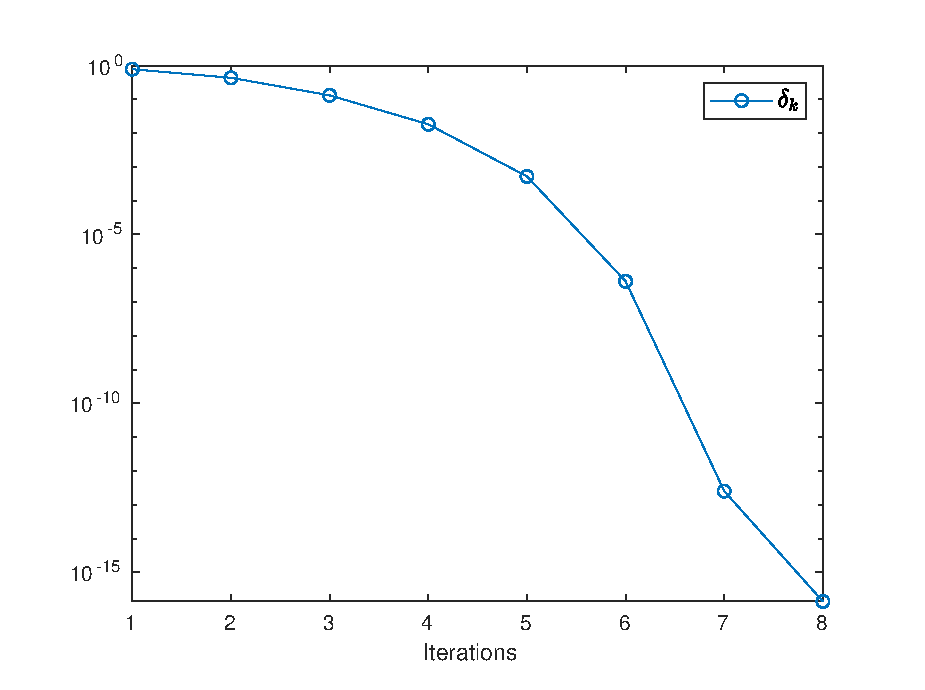
\includegraphics[scale=0.8]{hadamard}
  \caption{$\delta_k$ versus $k$ for the Hadamard matrix.}
  \label{fig:hadamard}    
\end{figure}

We finally include a routine to compute the square root of a symmetric positive
definite matrix by doing a Cholesky decomposition $A = R^*R$ and then performing
a polar decomposition.
Given $R = UH$, we then have $A = (UH)^*UH = H^*H = H^2$.
As seen in the case of the polar decomposition the algorithm is accurate for the
ill conditioned Hilbert matrix.
We have $\normo{A - \hat{H}^2}/\normo{A} = \num{5.7e-17}$.

\bibliographystyle{unsrt}
\bibliography{polar}

\end{document}
